\chapter{Aufbau \sppname}

\section{Architekturbeschreibung}

Sinn und Zweck des \gls{snort} \gls{praeprozessor}s \gls{sppname} ist das Abfangen,
Komprimieren und Weiterleiten von \gls{profinet}-\glspl{paket}n. Diese
sind durch \gls{ethertype} unterscheidbar. Er muss der Hexadezimalzahl 0x8892 entsprechen.
Hauptbestandteil des \gls{praeprozessor}s ist eine erweiterbare Baumstruktur von Decodern, welche rekursiv, Schicht für Schicht, ein \gls{paket} bearbeiten und benötigte Informationen in ein \gls{truffle} schreiben. Ein \gls{truffle} ist eine von uns vordefinierte Datenstruktur im \gls{praeprozessor}.
Pro Netzwerk-\gls{paket} entsteht ein \gls{truffle}, welches erheblich kleiner und kompakter als herkömmliche Netzwerkpakete sind. Dieses wird dann über den \gls{ipc}-Teil des \gls{praeprozessor}s
an \gls{programname} versendet, ????? um den Informationsfluss zu erhalten aber auch zu minimieren. SINN? ??????\newline
Zusätzlich kann mit einer selbst geschriebenen Datenstruktur ab diesem Zeitpunkt des Informationsflusses für einiges mehr an Sicherheit gesorgt werden.
Ein weiterer Vorteil der \glspl{truffle} ist die Gelegenheit für einen Sicherheitscheck bevor es gesendet wird. Wir wissen aufgrund der rekursiven Struktur unseres Decoder-Baums welche Daten wir zu erwarten haben. Sollte wir Inkonsistenzen feststellen, es ein Fehler vorliegen, oder etwas anderes keinen Sinn ergeben, so setzen wir im Truffle entsprechende Flags, damit \gls{programname} Statistiken für Auffälligkeiten einzelner Kommunikationsteilnehmer anfertigen kann.\newline
\gls{sppname} ist absichtlich klein gehalten, da es empfohlen wird \gls{snort}-\gls{praeprozessor}en nicht performance-lastig zu entwerfen. Der oben beschriebenen Ablauf findet sich als Sequenzdiagramm in Kapitel 4 !!!!! ref hinzufügen? !!!!!.


\section{UML-Diagramm}

\begin{sidewaysfigure}
  \centering
  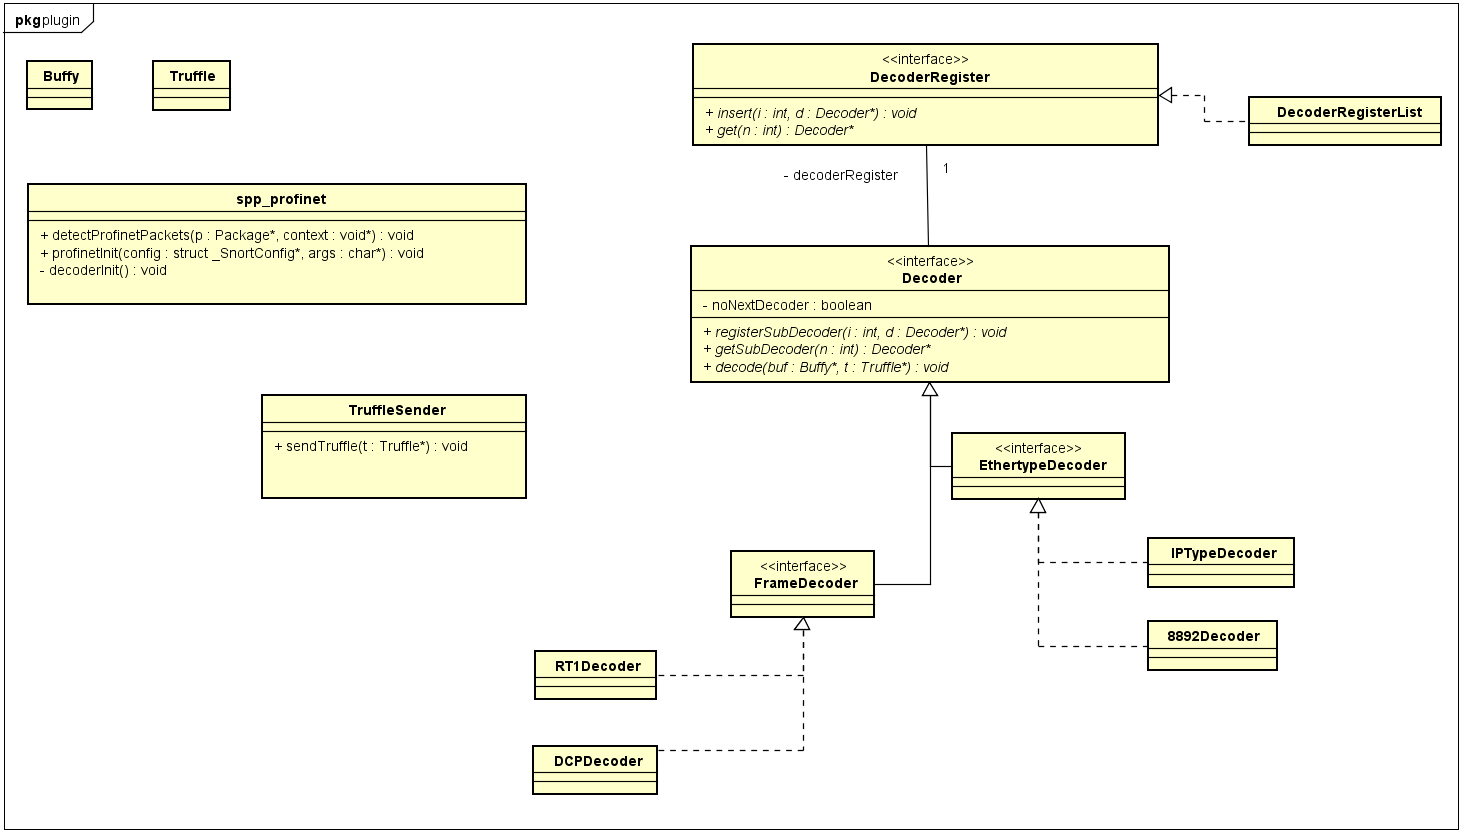
\includegraphics[width=\paperwidth]{../diagramimages/spp_profinet.png}
  \caption{\gls{praeprozessor} \gls{sppname}}
\end{sidewaysfigure}
